\chapter{Technicalities}
Not every placement of the vacancies in the unit cell will create a proper crystal when the translational symmetry is taken into account. For this to occur, it is required that the distance and angle between the vacancies is in accordance with the lattice vectors.

An example of this detail is that we cannot choose a unit super-cell of arbitrary order to create a Kagome lattice, only odd-order super-cells can create an exactly symmetric crystal as shown in Fig.~\ref{kagome}.
%~~~~~~~~~~~~~~~~~~~~~~~~~~ FIGURE ~~~~~~~~~~~~~~~~~~~~~~~~~%
\begin{figure}[h!]
  \centering
  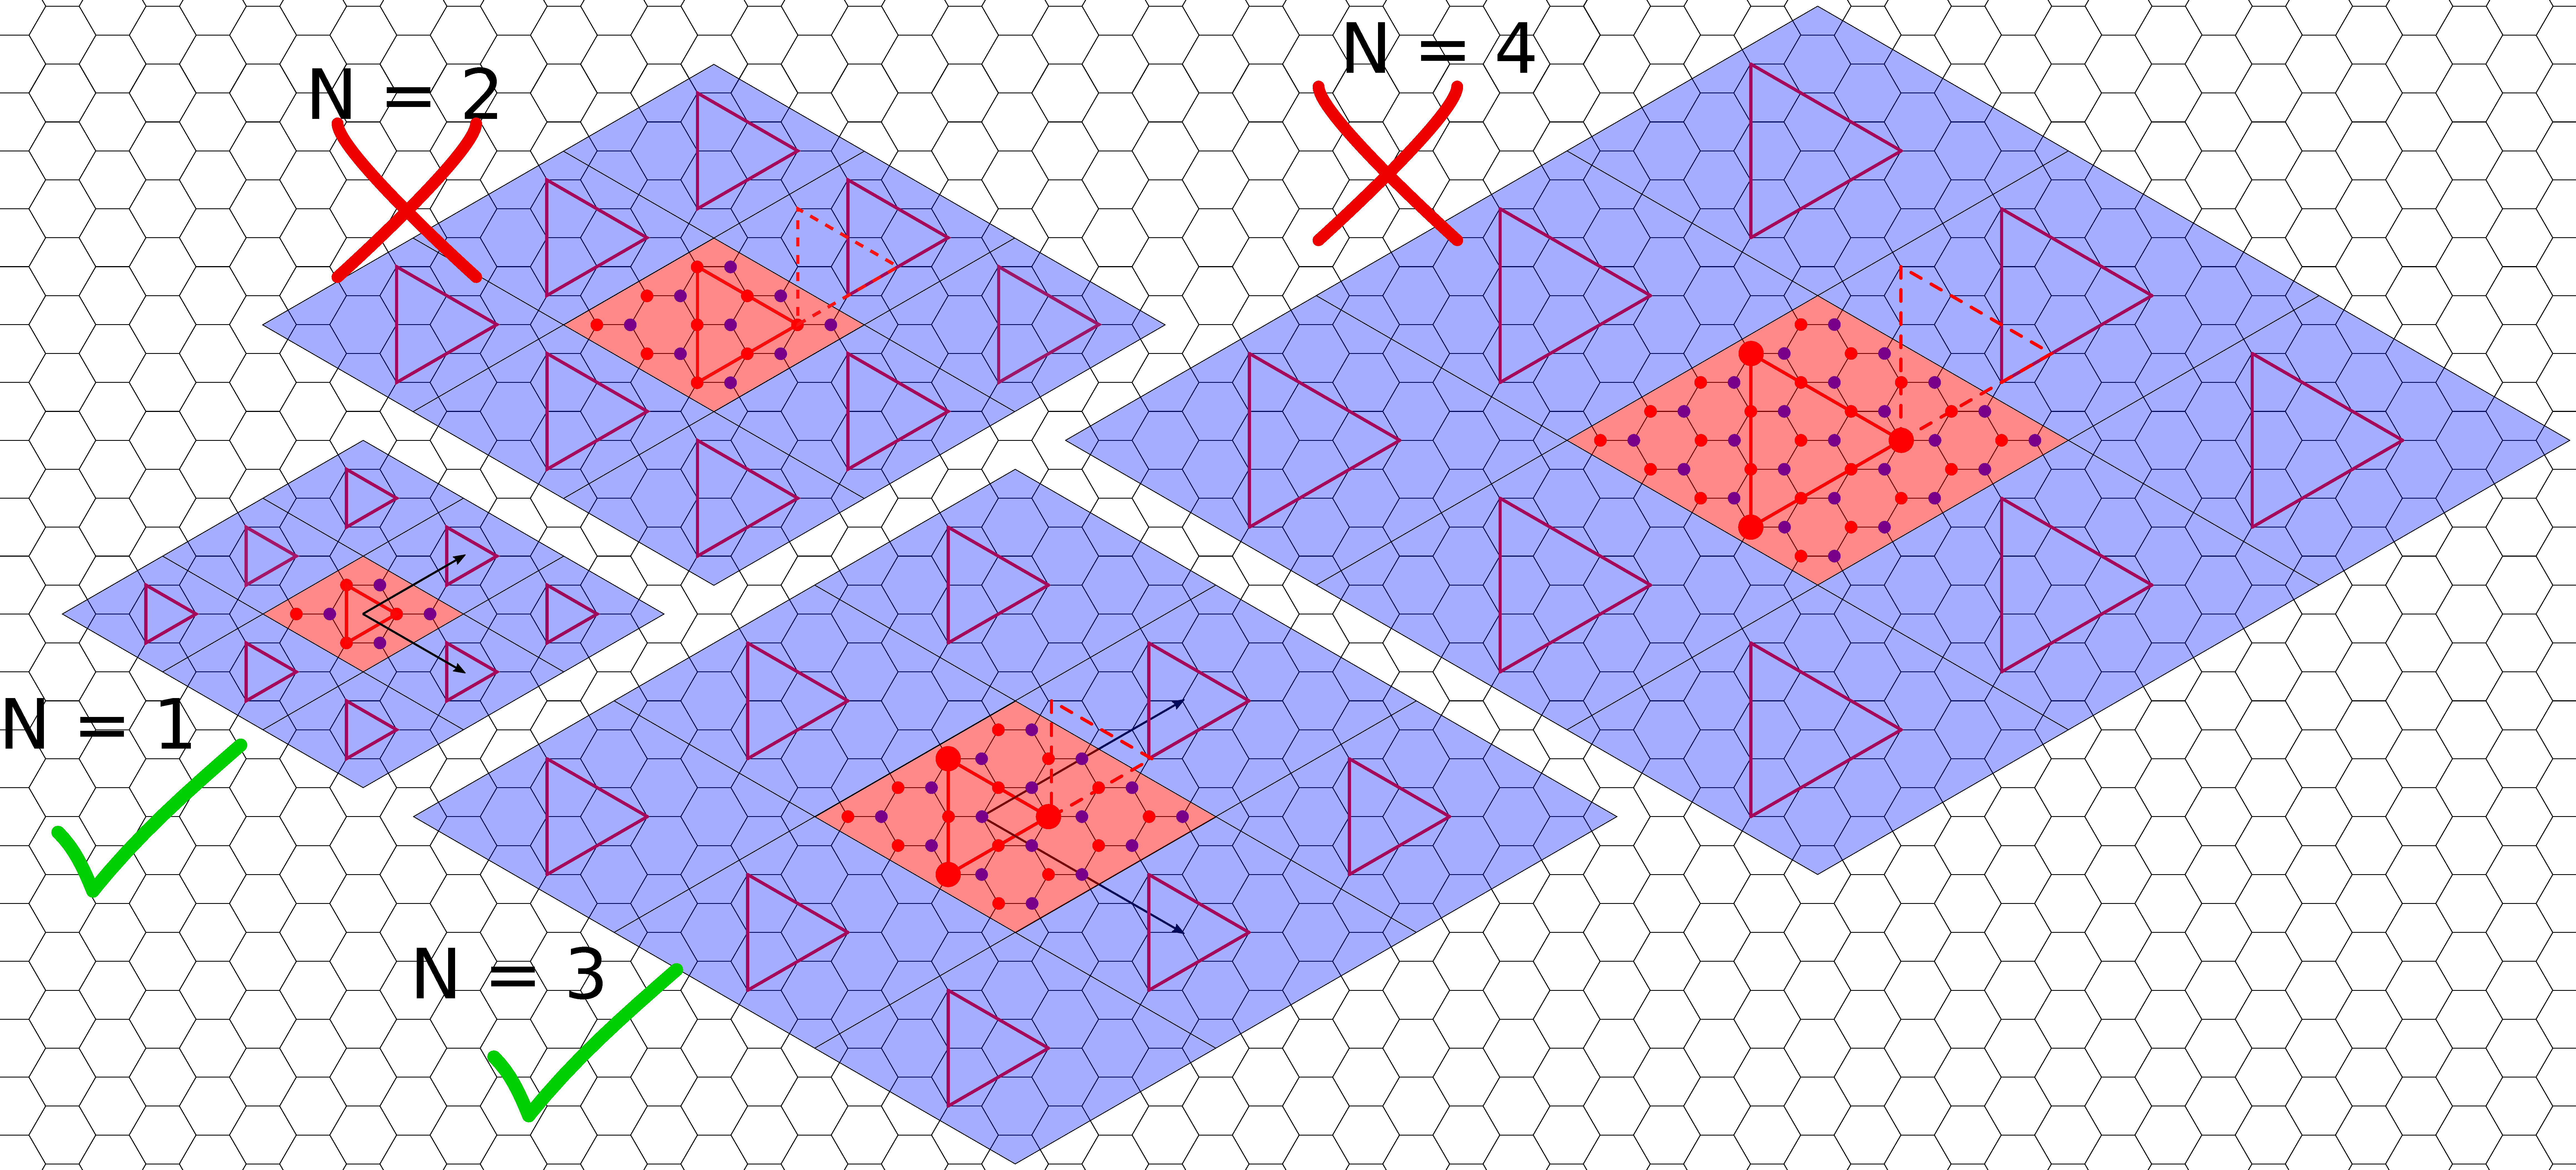
\includegraphics[width=0.6\textwidth]{artlat/fig/kagome_scale.pdf}
  \vspace{-5pt}
  \caption{The first examples for the simple supercell in graphene and its potential to host regular Kagome lattices}
  \label{kagome}
\end{figure}
\FloatBarrier
%~~~~~~~~~~~~~~~~~~~~~~~~~~~~~~~~~~~~~~~~~~~~~~~~~~~~~~~~~~~%
Nevertheless, this kind of inaccuracies will become more and more negligible as we user bigger and bigger unit cells.
In any case, these effect have only an anisotropic effect in the lattice, namely a small variation in the hoppings depending on the orientation.

The maximum anisotropy possible will be smaller than the size of a benzene ring (in fact it will be the distance of second neighbors in graphene $\sim\SI{2.1}{\angstrom}$). For this reason, and as long as we use a big enough system, we will neglect these small anisotropies.


\section{Models} %~~~~~~~~~~~~~~~~~~~~~~~~~~~~~~~~~~~~~~~~~~~~~~~~~~~~~~~~~~~~~%
\label{models}
\subsection{Triangular model}
The tight-binding model for a triangular lattice up to third neighbors is the following:
\begin{equation}
  \begin{split}
  H = H_0 +
      &t_1e^{-i\vec{k}\vec{a}_1} + t_1e^{-i\vec{k}\vec{a}_2} + t_1e^{-i\vec{k}(\vec{a}_1-\vec{a}_2)}+\\
      &t_2e^{-i\vec{k}(\vec{a}_1+\vec{a}_2)} + t_2e^{-i\vec{k}(2\vec{a}_1-\vec{a}_2)} +
      t_2e^{-i\vec{k}(-\vec{a}_1+2\vec{a}_2)}+\\
      &t_3e^{-i\vec{k}2\vec{a}_1} + t_3e^{-i\vec{k}2\vec{a}_2} + t_3e^{-i\vec{k}2(\vec{a}_1-\vec{a}_2)}+\\
      &c.c.
    \end{split}
\end{equation}
Which can be reduced to
\begin{equation}
  \begin{split}
  H = H_0 +
      &2t_1\left[cos(\vec{k}\vec{a}_1) + cos(\vec{k}\vec{a}_2) + cos(\vec{k}(\vec{a}_1-\vec{a}_2))\right]+\\
      &2t_2\left[cos(\vec{k}(\vec{a}_1+\vec{a}_2)) + cos(\vec{k}(2\vec{a}_1-\vec{a}_2)) +
      cos(\vec{k}(-\vec{a}_1+2\vec{a}_2))\right]+\\
      &2t_3\left[cos(\vec{k}2\vec{a}_1) + cos(\vec{k}2\vec{a}_2) + cos(\vec{k}2(\vec{a}_1-\vec{a}_2))\right]
    \end{split}
\end{equation}

\subsection{Graphene model}
\begin{equation}
  H = H_0 + H_1e^{-i\vec{k}\vec{a}_1} + H_2e^{-i\vec{k}\vec{a}_2}+
      H_{1-2}e^{-i\vec{k}(\vec{a}_1-\vec{a}_2)}+
      H_{12}e^{-i\vec{k}(\vec{a}_1+\vec{a}_2)} + c.c.
\end{equation}
where
\begin{equation}
  H_0 = \left(\begin{array}{cc}
    \epsilon_0 & t_1 \\
    t_1 & \epsilon_0
  \end{array}\right)\quad
  H_1 = H_2 = \left(\begin{array}{cc}
    t_2 & 0 \\
    t_1 & t_2
  \end{array}\right)\quad
  H_{1-2} = \left(\begin{array}{cc}
    t_2 & t_3 \\
    t_3 & t_2
  \end{array}\right)\quad
  H_{12} = \left(\begin{array}{cc}
    0 & 0 \\
    t_3 & 0
  \end{array}\right)
\end{equation}

\subsection{Kagome model}
The Kagome crystal is modeled with a triangular lattice with a three-atom basis as shown in Fig.~\ref{kagome_lat}

%~~~~~~~~~~~~~~~~~~~~~~~~~~ FIGURE ~~~~~~~~~~~~~~~~~~~~~~~~~%
\begin{figure}[h!]
\centering
  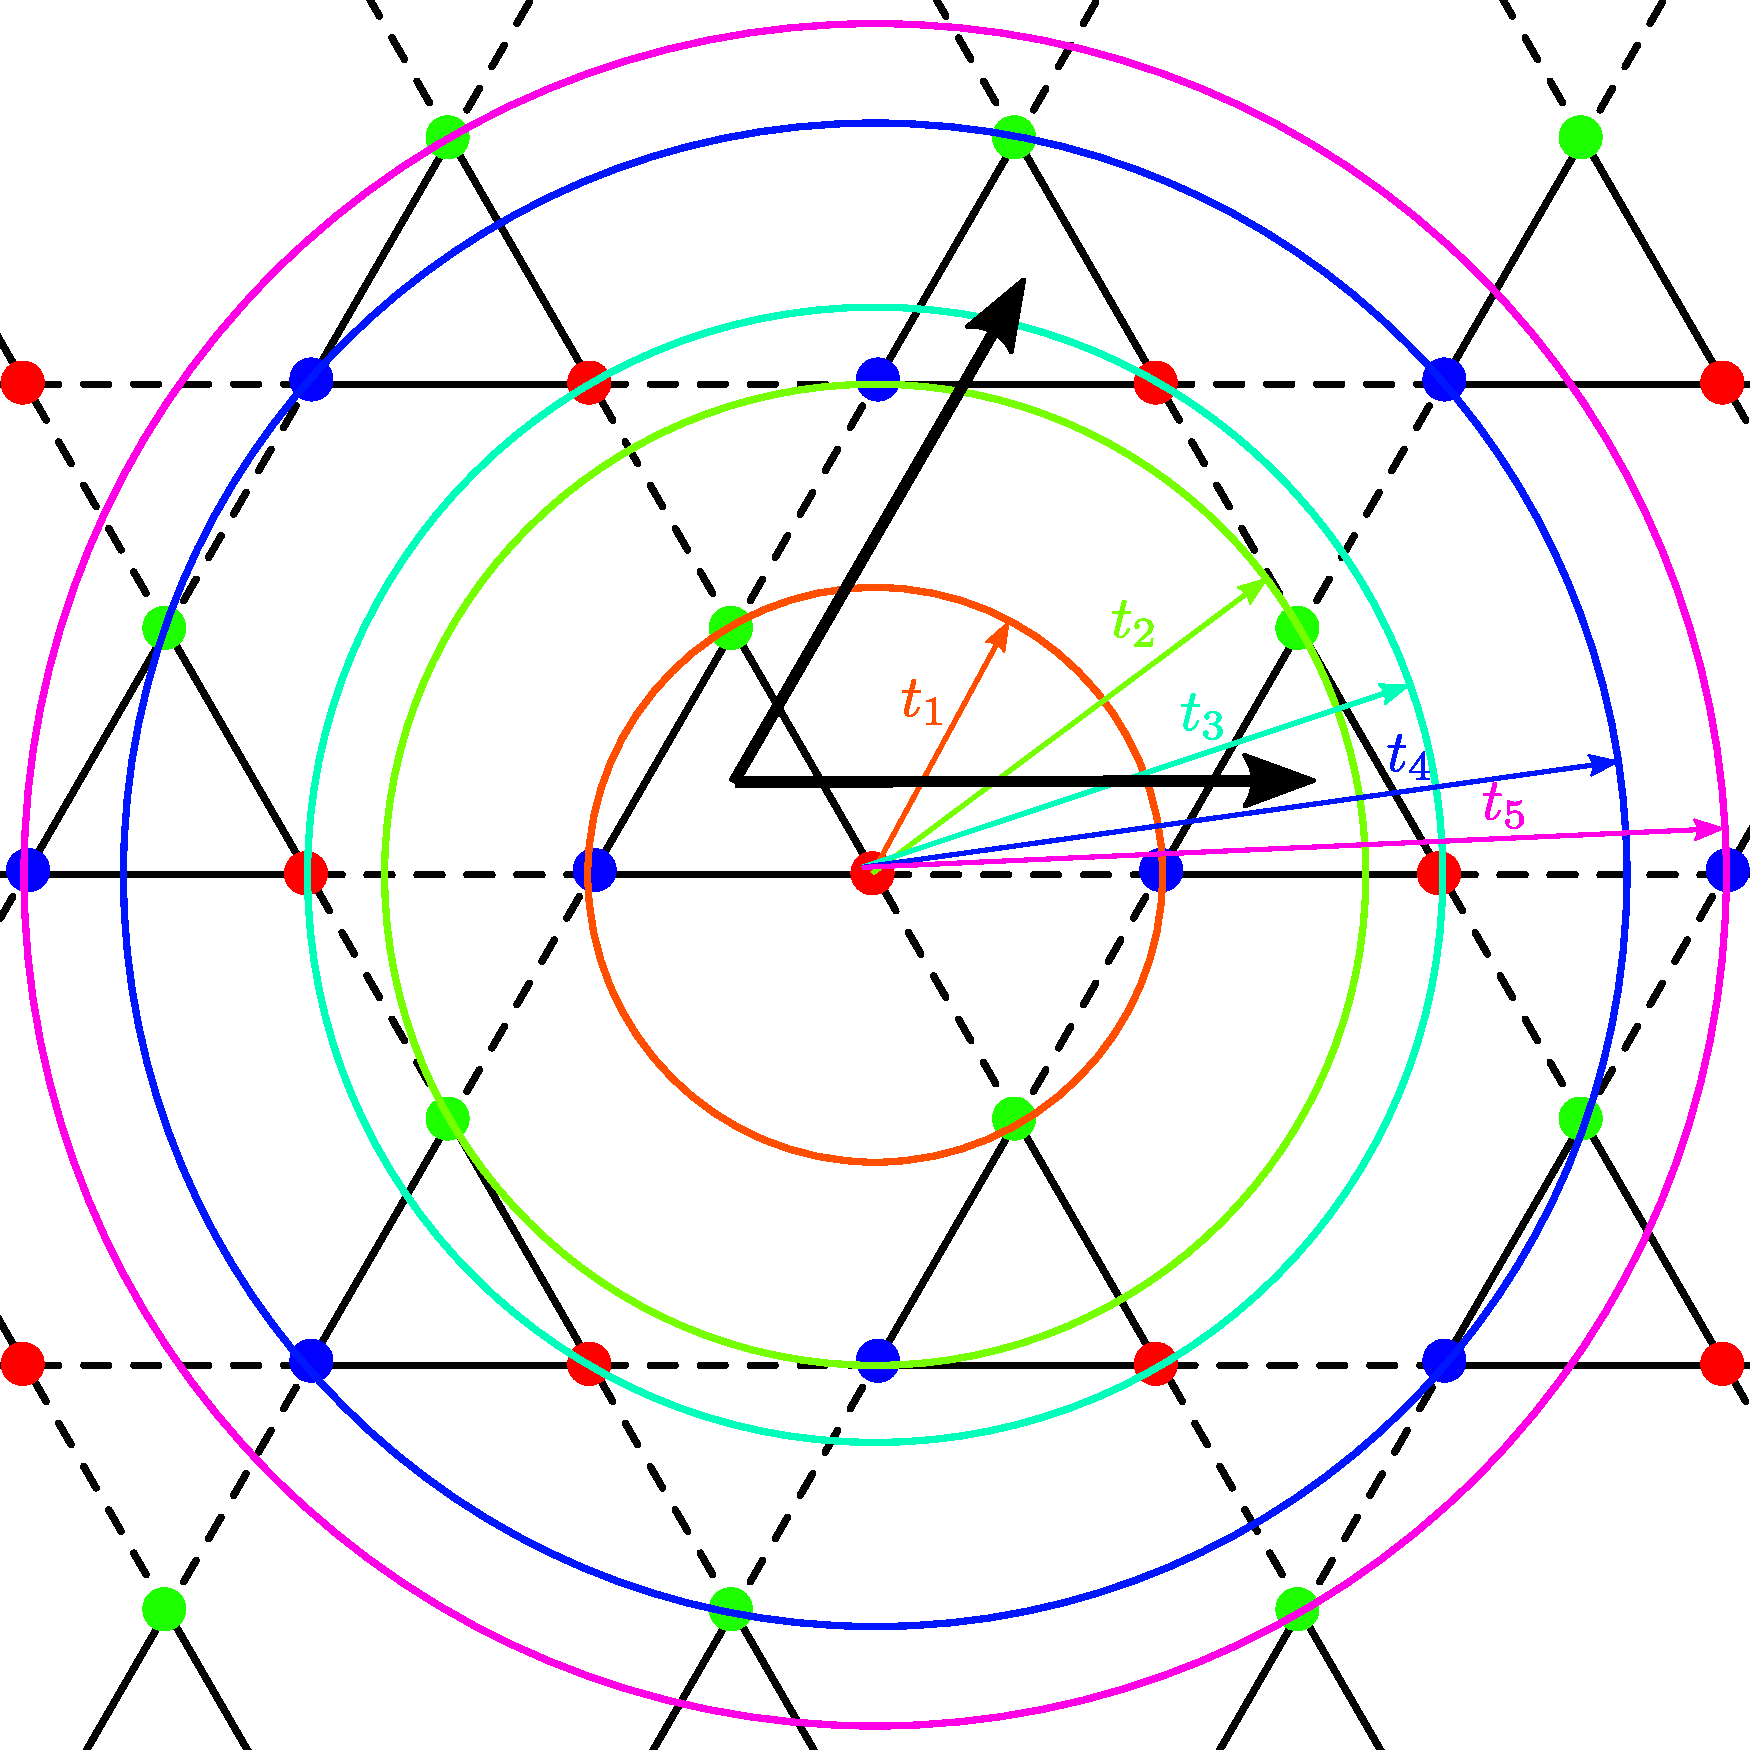
\includegraphics[width=0.6\textwidth]{artlat/fig/kagome_neighbors.pdf}
\vspace{-5pt}
\caption{Kagome crystal as a triangular lattice defined by the lattice vectors $\vec{a}_1$ and $\vec{a}_2$ and the three-atom basis shown by the red, blue and green atoms. The circles with radios labeled $t_1$, $t_2$... show the distances to neighbors of higher order.}
\label{kagome_lat}
\end{figure}
\FloatBarrier
%~~~~~~~~~~~~~~~~~~~~~~~~~~~~~~~~~~~~~~~~~~~~~~~~~~~~~~~~~~~%

The tight-binding Hamiltonian for this system considering up to third order neighbors consists of 4 terms:
\begin{equation}
  H(\vec{k}) = H_0 + H_1e^{-i\vec{k}\vec{a}_1} + H_2e^{-i\vec{k}\vec{a}_2} +
  H_{1-2}e^{-i\vec{k}(\vec{a}_1-\vec{a}_2)} + c.c.
\end{equation}
where the intra-cell hopping matrix is:
\begin{equation}
  H_0 = \left(\begin{array}{ccc}
  \varepsilon_0 & t_1 & t_1 \\
  t_1 & \varepsilon_0 & t_1 \\
  t_1 & t_1 & \varepsilon_0
  \end{array}\right)
\end{equation}
and the inter-cell hopping matrices are:
\begin{equation}
  H_1 = \left(\begin{array}{ccc}
    t_3 & t_2 & t_1 \\
    t_4 & t_3 & t_2 \\
    t_5 & t_4 & t_3
  \end{array}\right)\quad ; \quad
  H_2 = \left(\begin{array}{ccc}
    t_3 & t_4 & t_2 \\
    t_2 & t_3 & t_1 \\
    t_4 & t_5 & t_3
  \end{array}\right)\quad ; \quad
  H_{1-2} = \left(\begin{array}{ccc}
    t_3 & t_1 & t_2 \\
    t_5 & t_3 & t_4 \\
    t_4 & t_2 & t_3
  \end{array}\right)
\end{equation}
Note that up to $t_5$ hoppings are included for the sake of completeness but in order to include $t_4$ and $t_5$ the cell placed at $\vec{a}_1 + \vec{a}_2$ should also be considered. For this reason we will consider $t_4 = t_5 = 0$.

We begin to analyze the system by comparing the band structure with and without second neighbors.
